\chapter{Teorie}
Teoretická část práce se skládá ze~ dvou částí. První část věnuje popisu fungování kruhových podpisů obecně a druhá část se věnuje kryptografii založenou na mřížkách, které jsou odolné vůči kvantové kryptografii.

\section{Kruhové podpisy}

Metoda kruhového podpisu byla vytvořena v~roce 2001 skupinou Ronald L. Rivest, Adi Shamir a Yael Tauman. Výhoda kruhových podpisů je, že poskytují anonymitu členům skupiny při podepisování zpráv, dále jejich nezapomenutelnost a odolnost vůči kolizím. Během podepisování zprávy nejsme schopni zjistit, kdo jako první podepsal zprávu a kdo jako poslední, protože se jednotlivé zprávy na sebe odkazují a jeví se jako dokonalý kruh. Ani lidé z~podepisující skupiny neví, kteří další členové a v~jakém pořadí podepsali zprávu.

V~kruhovém podpisu má každý člen vlastní pár asymetrických klíčů (tedy soukromého a veřejného klíče). V~případě, že by jeden člen skupiny chtěl podepsat zprávu, musí vybrat členy skupiny, kteří zprávu podepíší (nemusí to být všichni členové skupiny, ale čím méně členů tím vyšší pravděpodobnost tipnutí si původci zprávy) a následně vykonat následující kroky. 

Vytvořit si náhodnou inicializační hodnotu \emph{u}. Vytvořit si šifrovací klíč z hashe původní zprávy $E = H(\mathrm{zpráva})$. Vytvoří si původní hodnotu \emph{v}, ze šifrovacího klíče a inicializační hodnoty $v = E(u)$, kterou bude využita dále. Vytvořit podepsání zprávy dalšími členy skupiny a to vytvořením náhodné hodnoty $x_i$, které umocníme veřejným klíčem člena skupiny $v = E(x_1^{pk_1})$ a použijeme exkluzivní disjunkci s~původní hodnotou \emph{v}. Tento krok se opakuje dokud nezbývá podpis pouze uživatele, který tuto operaci začal. Poslední krok vykoná uživatel vypočtením poslední hodnoty \emph{v}~pomocí exkluzivní disjunkce s~inicializační hodnotou, kde výsledek umocní na svůj soukromý klíč $v = E(u \oplus v)^{sk}$. Po vytvoření všech potřebných hodnot uživatel odešle původní zprávu, hodnotu $v$, včetně vygenerovaných náhodných $x_i$ hodnot uživatelů a veřejné klíče uživatelů.

Pro ověření zprávy, že opravdu pochází ze skupiny z~jaké se vydává. Uživatel pro ověření použije stejné kroky při šifrování kromě poslední kroku, který je jemně pozměněn. V~posledním kroku bude poslední hodnotu umocňovat veřejným klíče jednoho z~podepisujících (nezáleží na pořadí v~jakém ověřující člověk informace potřebné k~ověření) $v = E[(u \oplus v)^{sk}]^{pk}$, díky matematice v~pozadí těchto operací se ověří díky XOR operacím, že se jedná opravdu o~podpis některého z~uživatelů skupiny \cite{Buchanan}.

\begin{figure}[htbp]
  \centering
  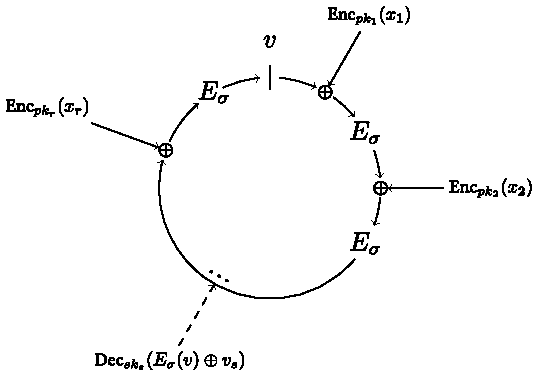
\includegraphics[width=0.7\textwidth]{img/ring_signature.pdf}
  \caption{Ukázka kruhového podpisu \cite{Ring signature picture}.}
  \label{Ring signature}
\end{figure}


\section{Kryptografie založená na mřížkách}

Metoda kterou jsme implementovali v této práci využívá mřížky, což jsou množiny bodů v n-rozměrném prostoru uspořádány periodicky. Využívají dvou matematických problémů, které jsou imunní vůči kvantovým počítačům. Máme soubor lineárně nezávislých vektorů, které generují mřížku.

Prvním problémem je problém nejkratšího vektoru (Shortest Vector Problem - SVP). Problematikou je hledáním nejkratšího vektoru báze, který patří do dané mřížky. Součásti problému je také nalezení co nejmenšího vektoru, který není nulový. Druhým problémem je nalezení nejbližšího vektoru, což je spojeno s~nalezením nejbližšího libovolného vektoru v~mřížce. Zde je možné, aby nalezený vektor byl nulový a zároveň byl nejblíže zvolenému bodu (Closest vector problem - CVP). Naše vybrané schéma právě využívá problém nejkratšího vektoru (SVP).


\section{Jiné druhy podpisů}

Existuje spousta různých druhů post kvantových algoritmů pro samotné podpisy. Níže uvedené jsou často používané na podepisování. 

\begin{itemize}
  \item Hash-and-sign,
  \item Bimodal Lattice Signature Scheme (BLISS),
  \item Goldreich-Goldwasser-Halevi (GGH),
  \item NTRU Signature Algorithm,
\end{itemize}

\hfill

Zároveň jsme uvedené algoritmy posloužili jako inspirace pro námi vybraného algoritmu, který byl v~této práci implementován. Post kvantová kryptografie není zase až tak rozšířená takže počet kruhových post kvantových podpisu je menší. Zde jsou uvedeny všechny ostatní kruhové podpisy které jsme zvážili na implementaci.

\begin{itemize}
  \item Lattice-based Linkable Ring Signature with Co-Signing (L2RS-CS) \cite{Torres2020}.
\end{itemize}


\begin{figure}[htbp]
  \centering
  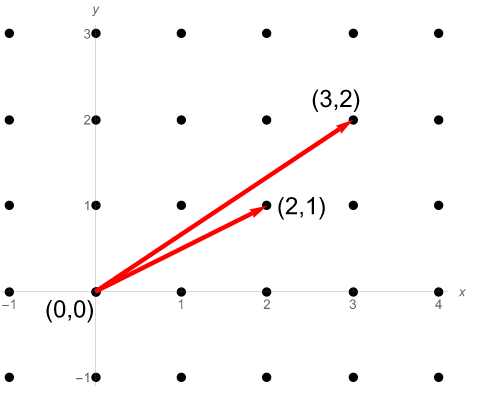
\includegraphics[width=0.7\textwidth]{img/mrizky.png}
  \caption{Ukázka kryptografie na mřížkách \cite{Mrizky picture}.}
  \label{lattice}
  \label{Ring signature}
\end{figure}

test
test
test